\section{Experimental evaluation}
\label{Sec:experimental-eval}

Here we report the result of the tests executed to compare the performance between the sequential and parallel version of the A-Star implementation.\\
To test the parallel A* algorithm we changed the number of threads and the function used to compute the recipient (\ref{compute_reci}). \\
All the tests are performed on a Linux environment.

\subsection{Time performance}


\subsubsection{Grid Milan}
The graph generated from the grid of Milan (1024x1024) has around 800k nodes and has random generated weights to increase the difficulty to find the path with the best cost.

\begin{center}
    
    \begin{minipage}[b]{0.3\textwidth}

            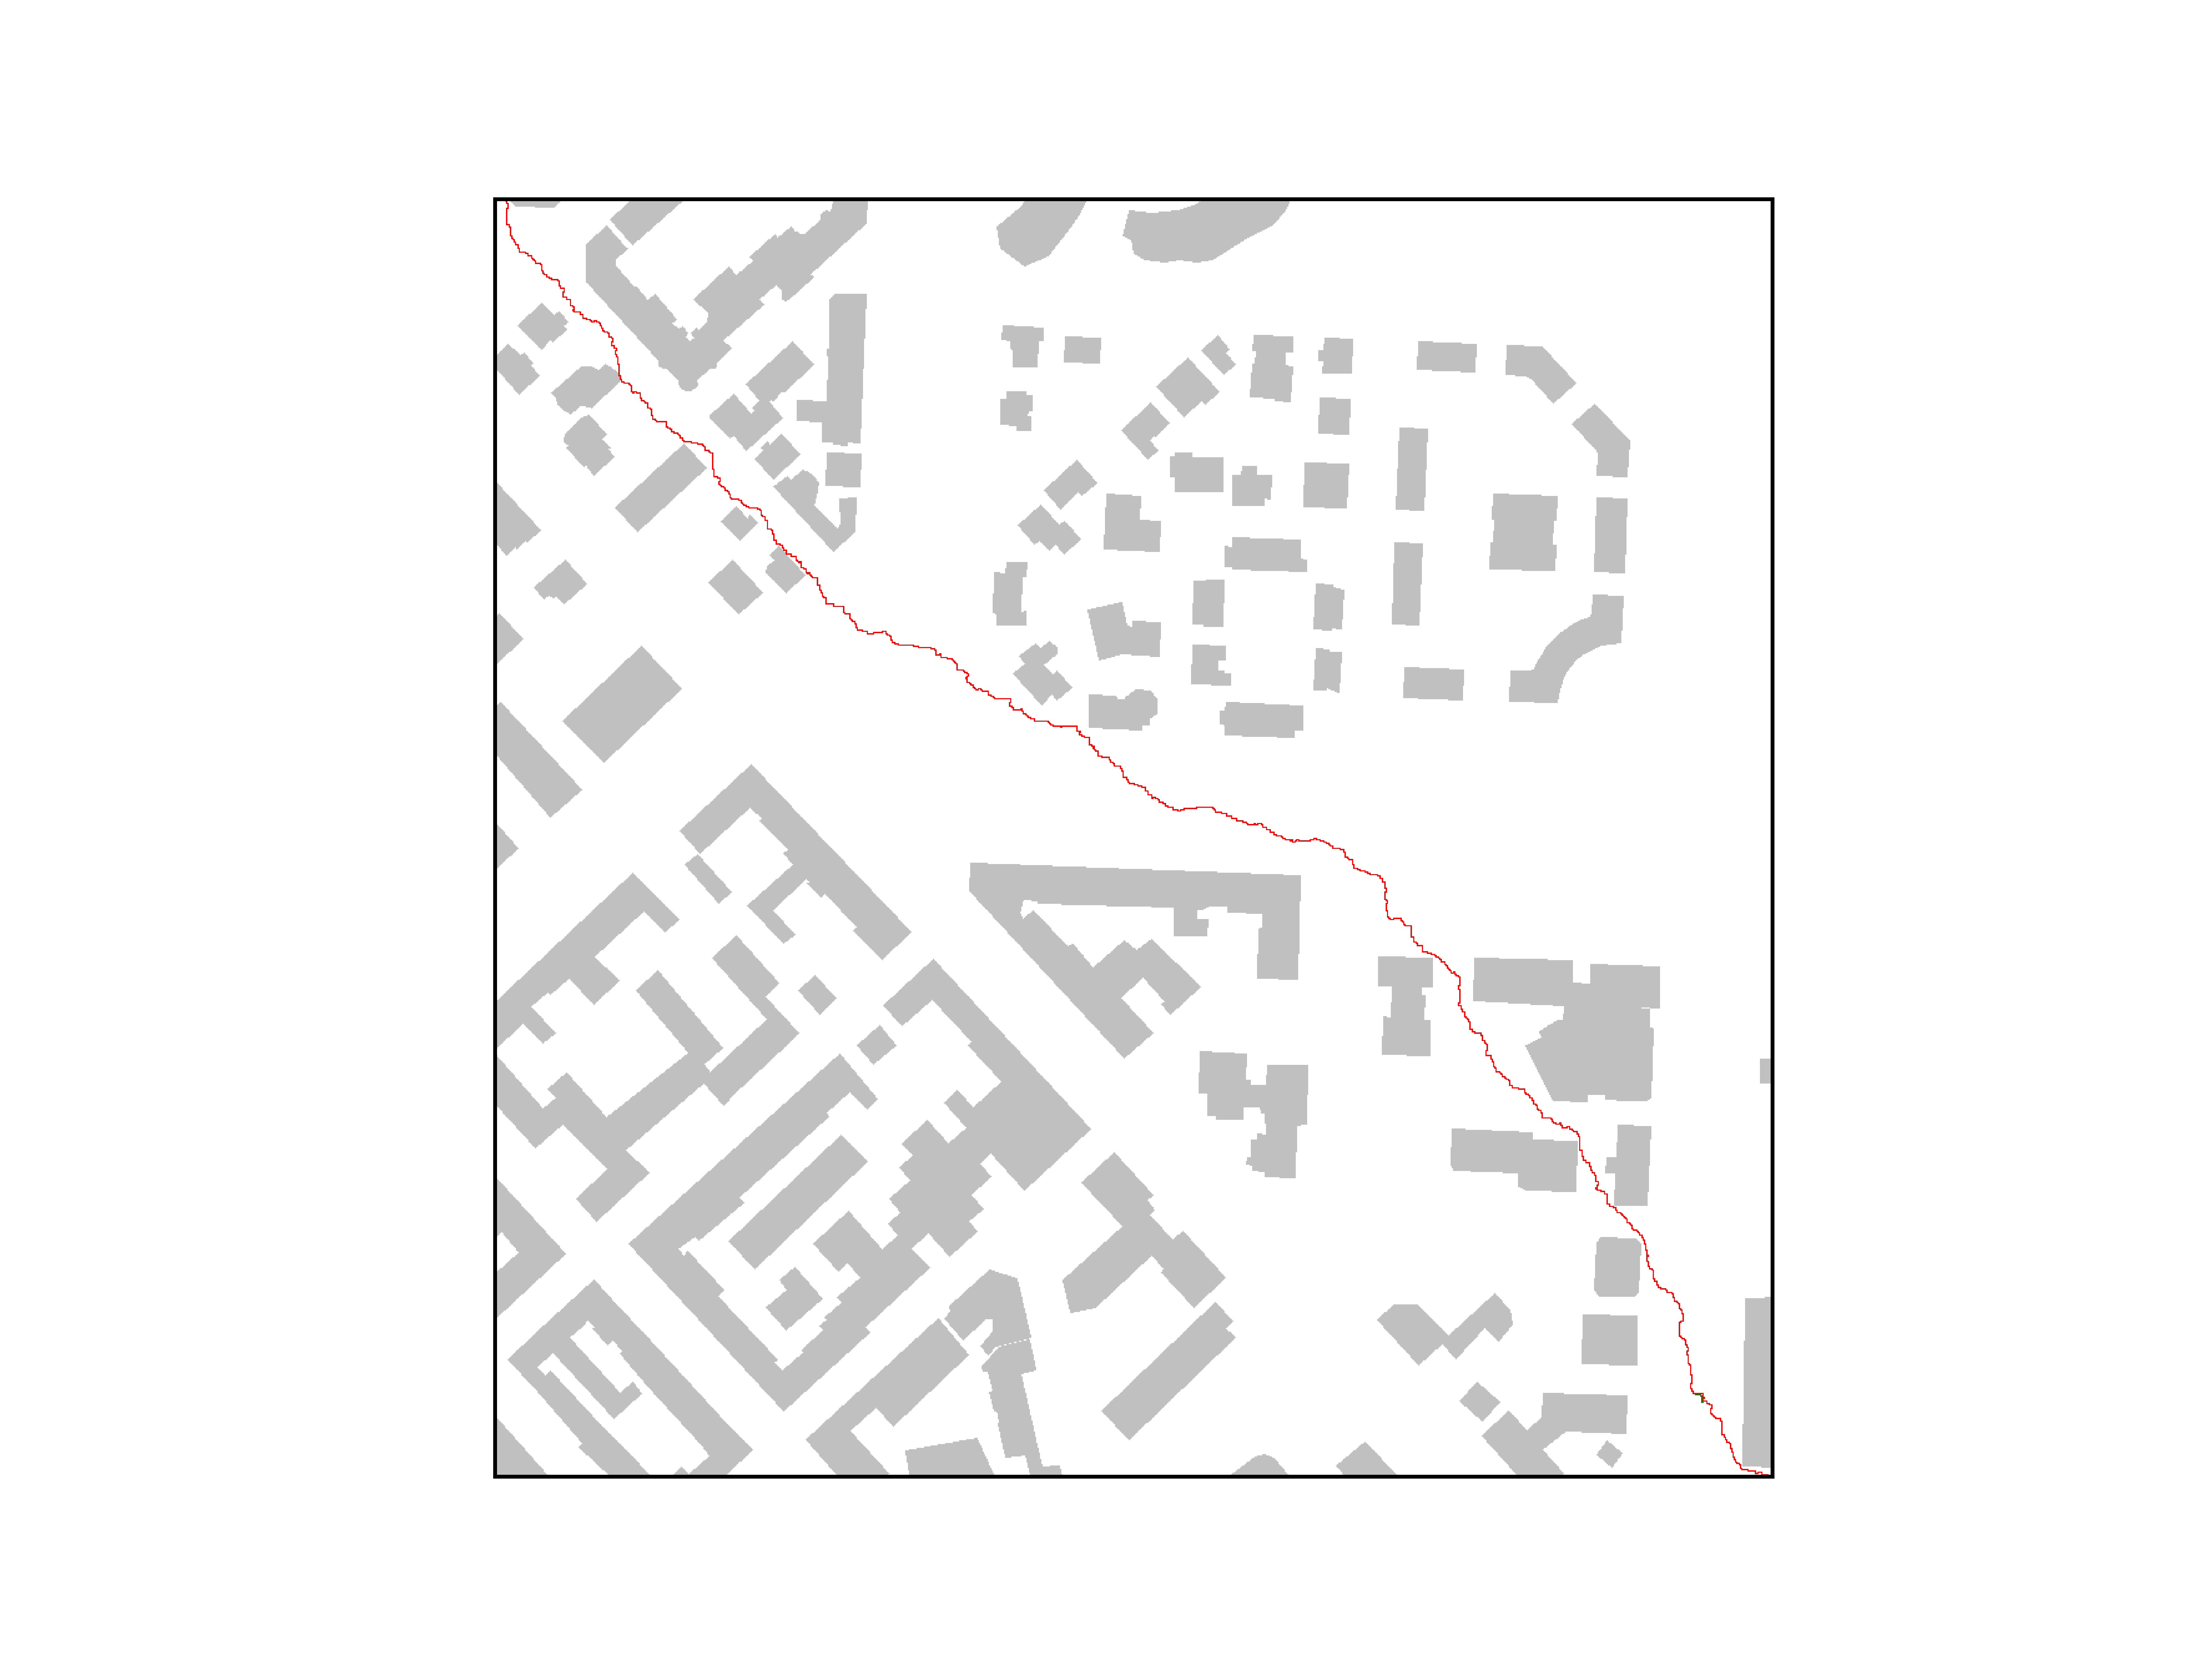
\includegraphics[scale=0.5]{gridMilan.png}
            \captionof{figure}{Milan map with path found}
            \label{Milan-grid}
        
    \end{minipage}%
    \begin{minipage}[b]{0.6\textwidth}
        
            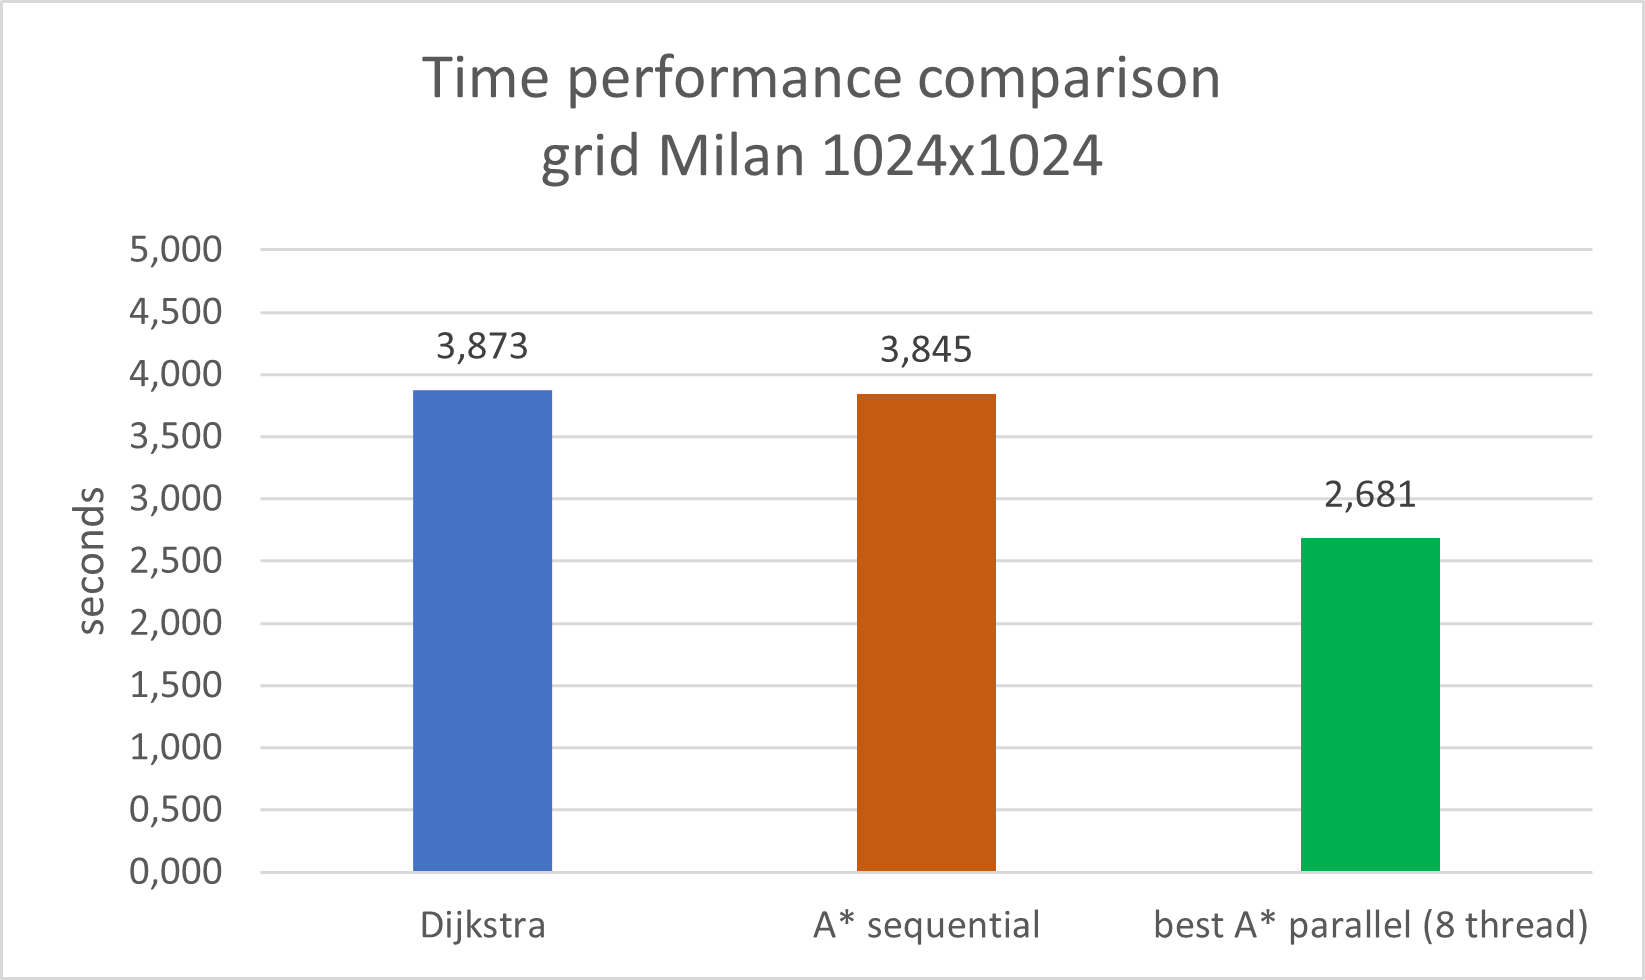
\includegraphics[scale=0.7]{milanComparison.png}
            \captionof{figure}{Performance comparison on different algorithms}
            \label{Milan-comp}
    \end{minipage}
    
\end{center}


\begin{figure}
    \centering
    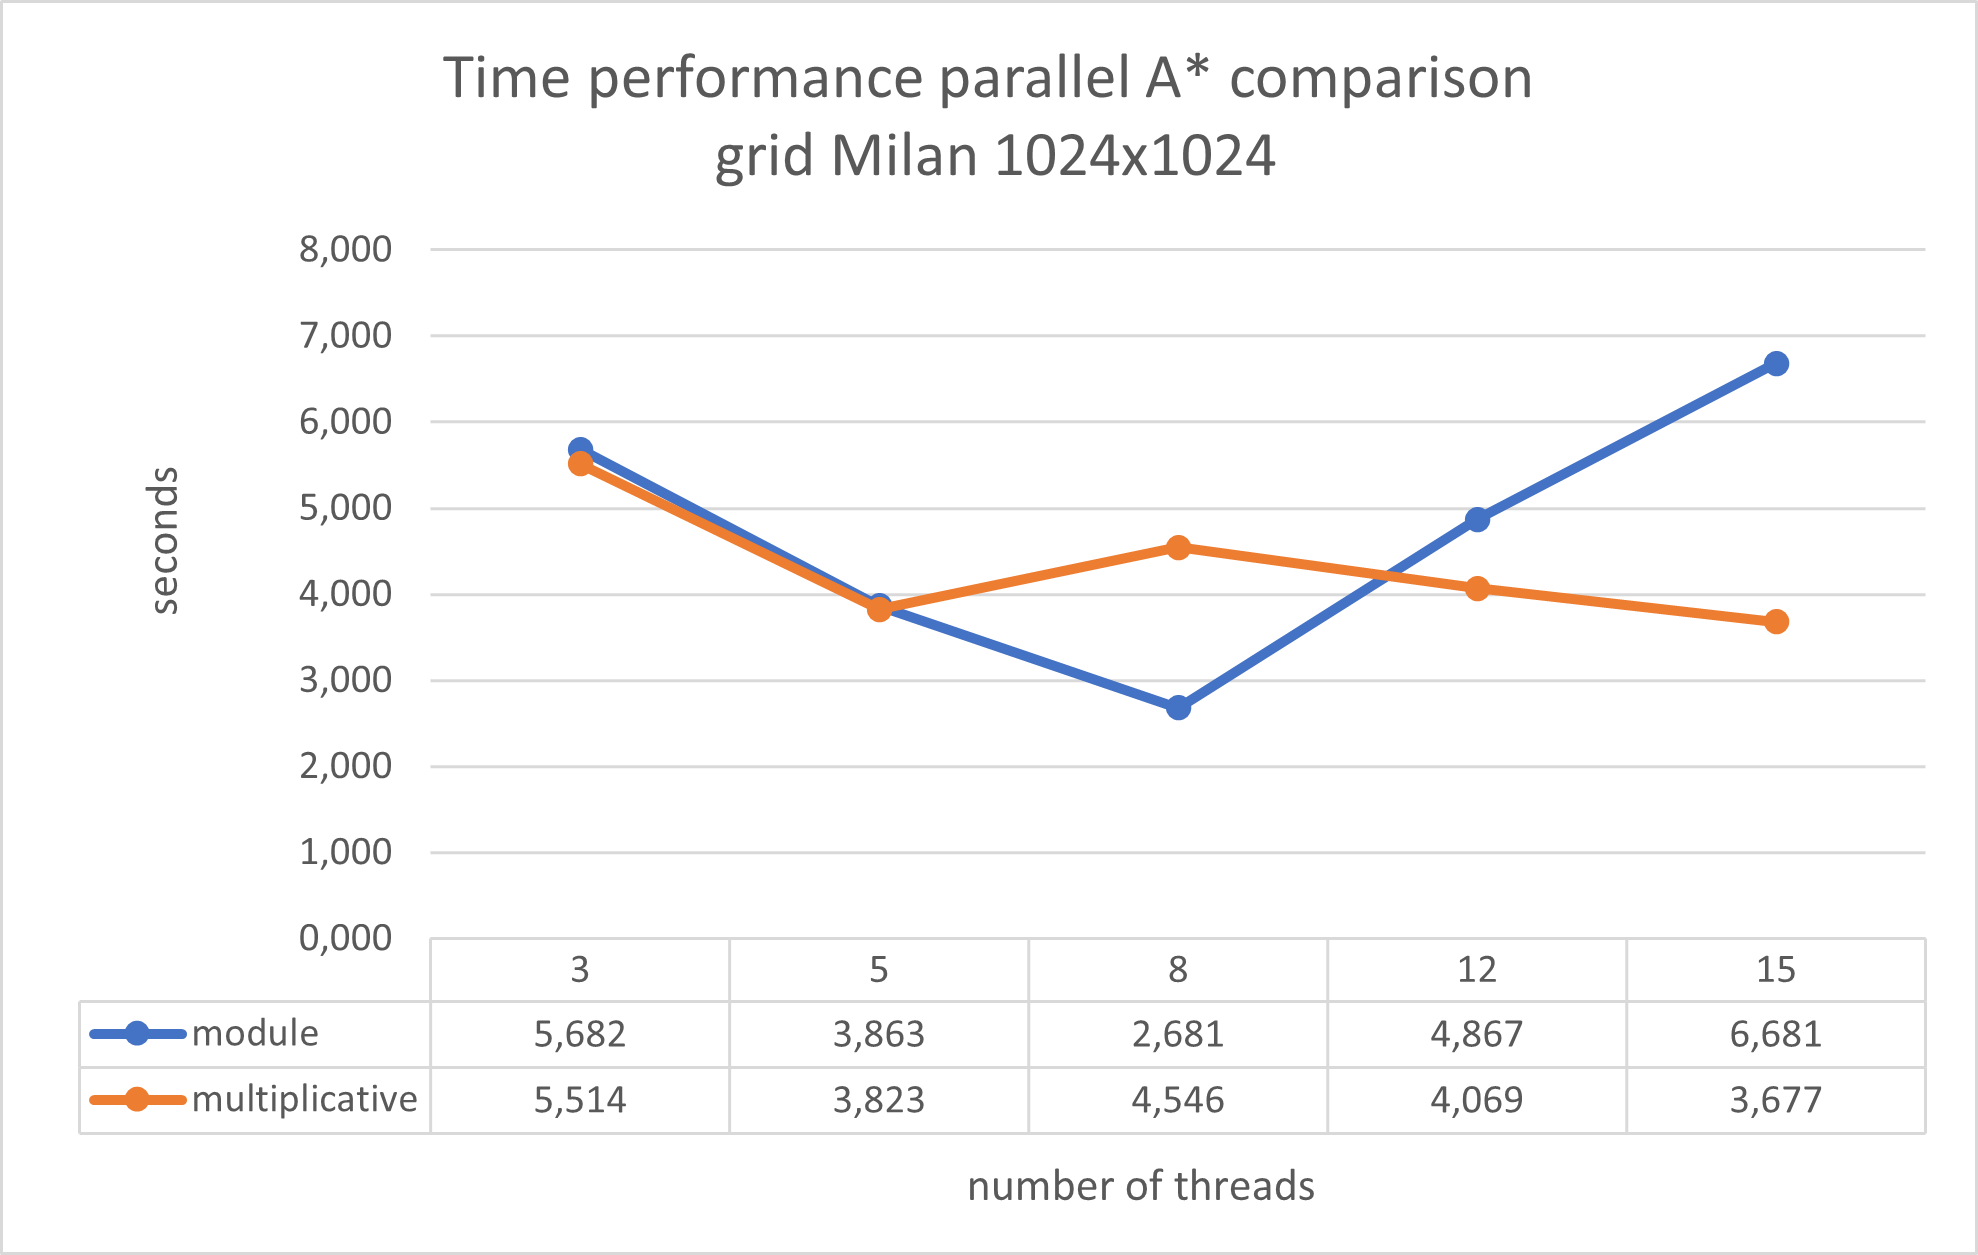
\includegraphics[scale=0.7]{milanParComparison.png}
    \caption{Performance comparison on different thread number and compute recipient function}
    \label{Milan-par-comp}
\end{figure}


Looking at Figure \ref{Milan-comp}, and taking into account that we chose the most efficient number of threads for parallel A*,
we can notice a better performance compared to the sequential A* and the Dijkstra algorithms. 
To find the best result we tried the parallel A* changing the number of threads and the compute recipient function:
the Figure \ref{Milan-par-comp} shows all the experimental results of the tests.
\\
Comparing the two compute recipient functions (simple module and multiplicative hash)
on this relative small graph, it can be observed that when runnig with limited number of threads the performance are similar.
When increasing the level of parallelism the performances are no loger comparable, and the algorithm with the multiplicative hash function is faster.


\subsubsection{Large Map}

To test more our algorithms we used larger graphs, always with random weights, with about 4 Millions nodes.

\begin{figure}
    \centering
    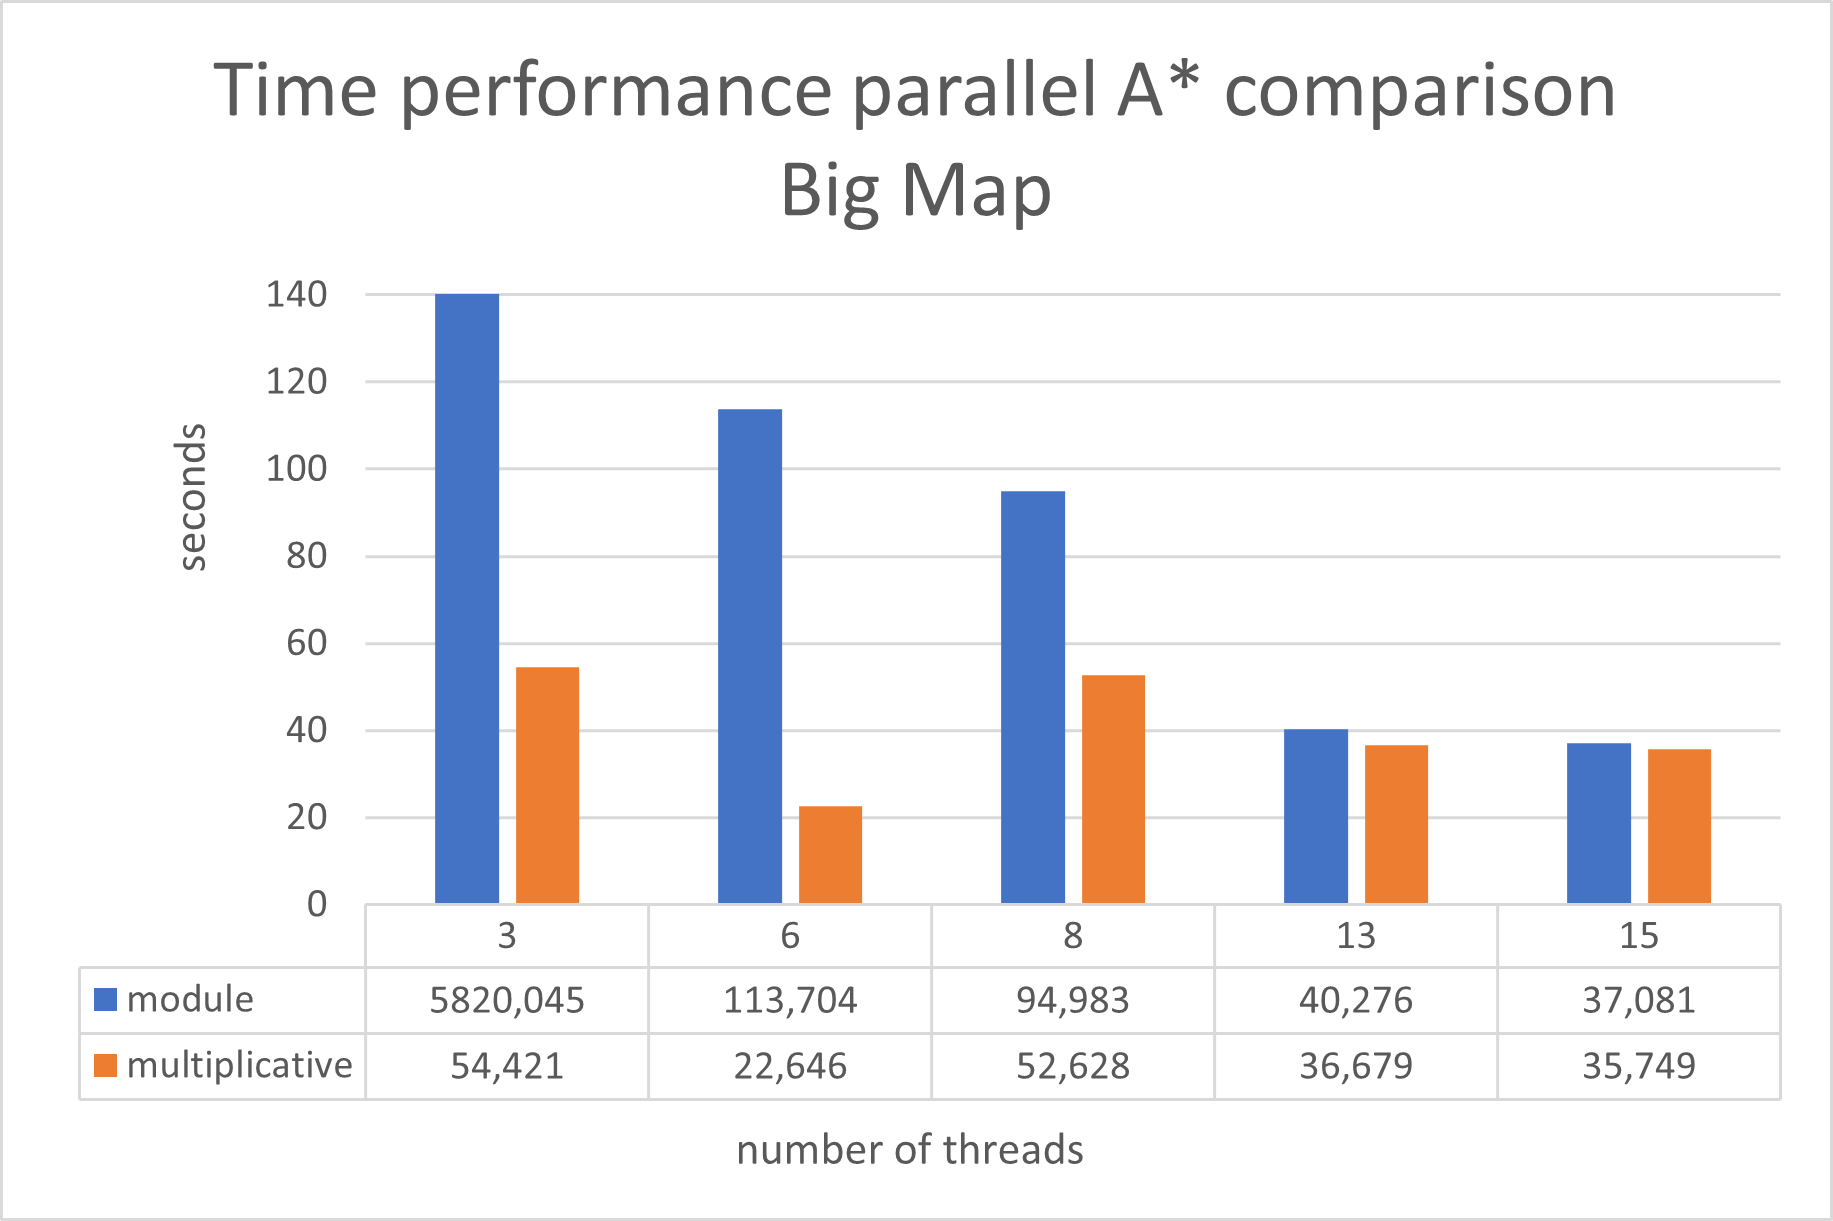
\includegraphics[scale=0.7]{mapParComparison.png}
    \label{Map-par-comp}
    
    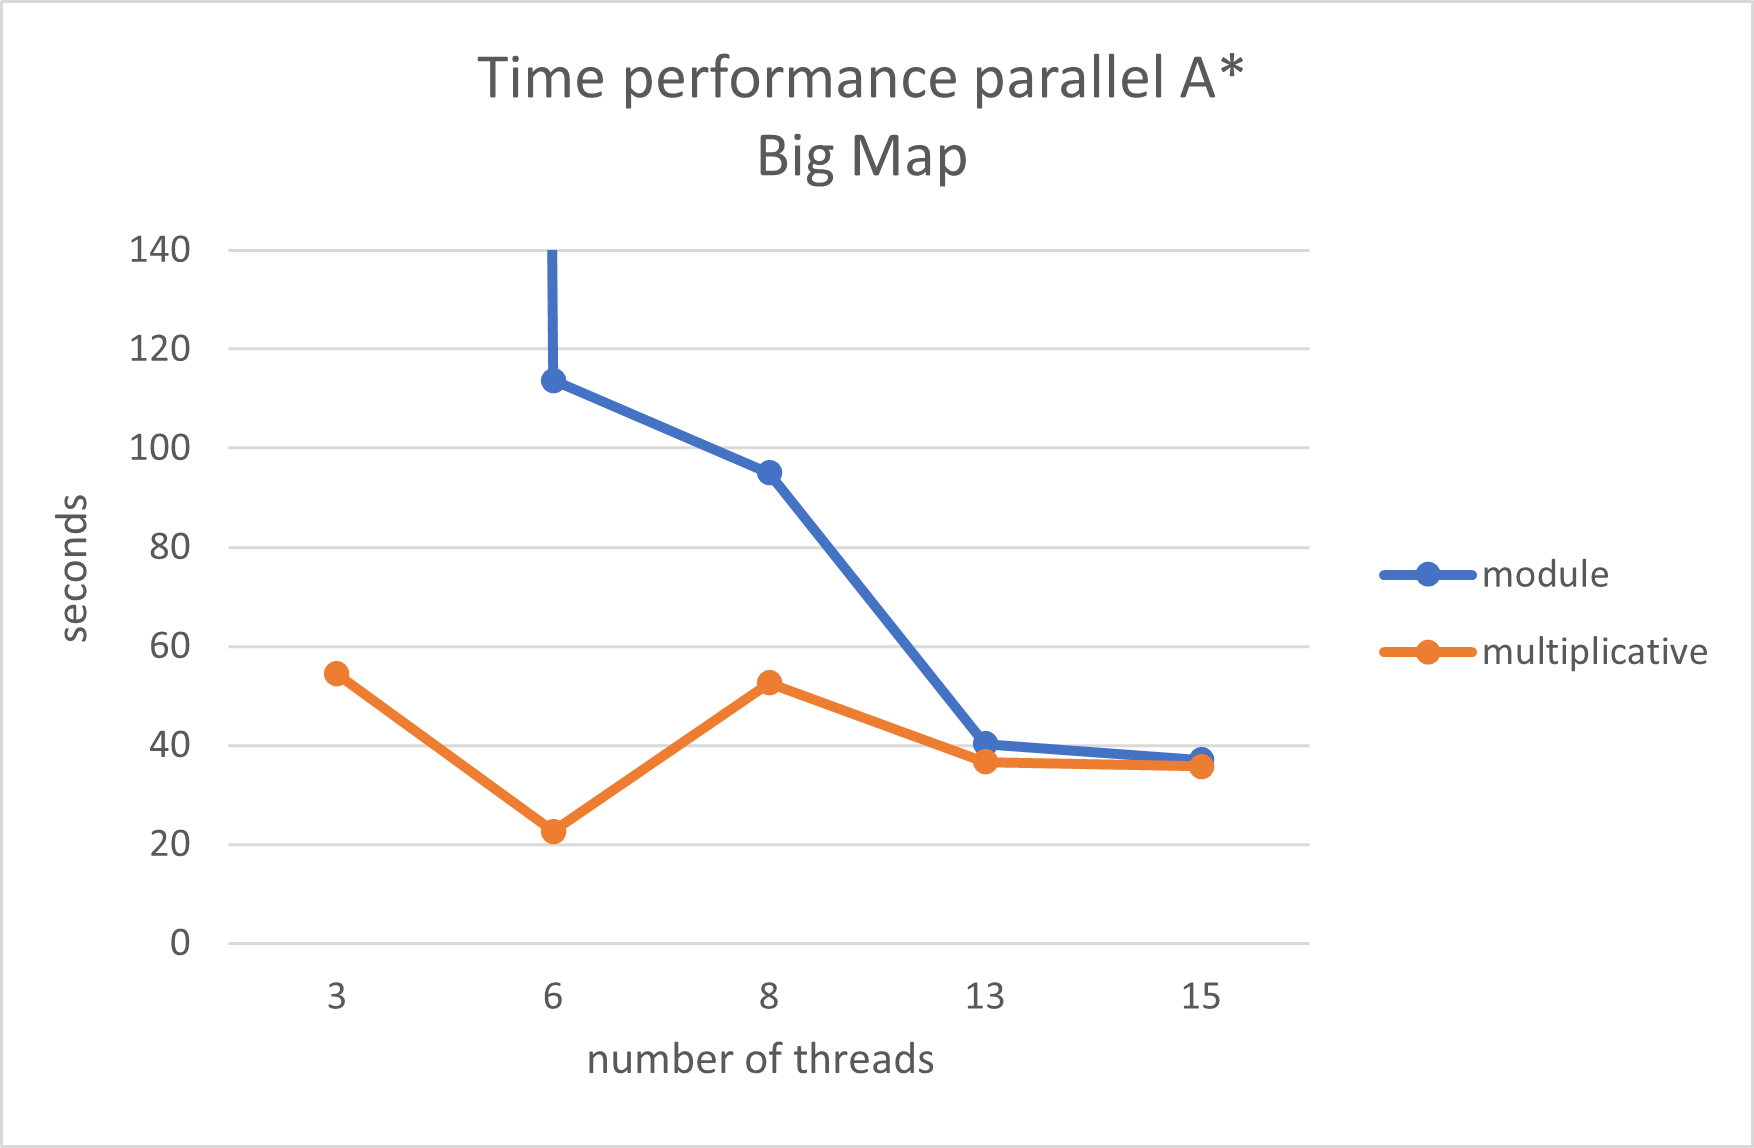
\includegraphics[scale=0.7]{mapParComparisonLines.png}
    \label{Map-par-comp-lines}
    \caption{Performance comparison on different thread number and compute recipient function}
\end{figure}


By looking at the results on Figure \ref{Map-par-comp}, it can be observed that the multiplicative hash function is more stable when changing the number of threads.
For small level of parallelism (eg. 3 threads) the module hash needs almost two hours to found the correct path, while exploring and revisiting a large number of nodes.
The seconds needed to find a path decreses considerably with the increasing of the number of threads, but for some value (mostly even values of threads eg. 12), the time to converge to a result greaty increases again.
The multiplicative hash instead, has generally better performances, but we found some limits on the number of threads (again even values from 16 onwards) beyond which the time increases.


\subsection{memory occupation}

To track the memory occupation we used the Valgrind-Massif tool which is a heap profiler. It measures how much heap memory the program uses: this includes both the useful space,
and the extra bytes allocated for book-keeping and alignment purposes.
\\
The graph generated shows the memory occupation on specific time snapshots. The X axis indicates the bytes allocated/deallocated on the heap and stack(s), while the Y axis shows the actual memory occupation on that specific snapshot.


\begin{figure}
    \centering
    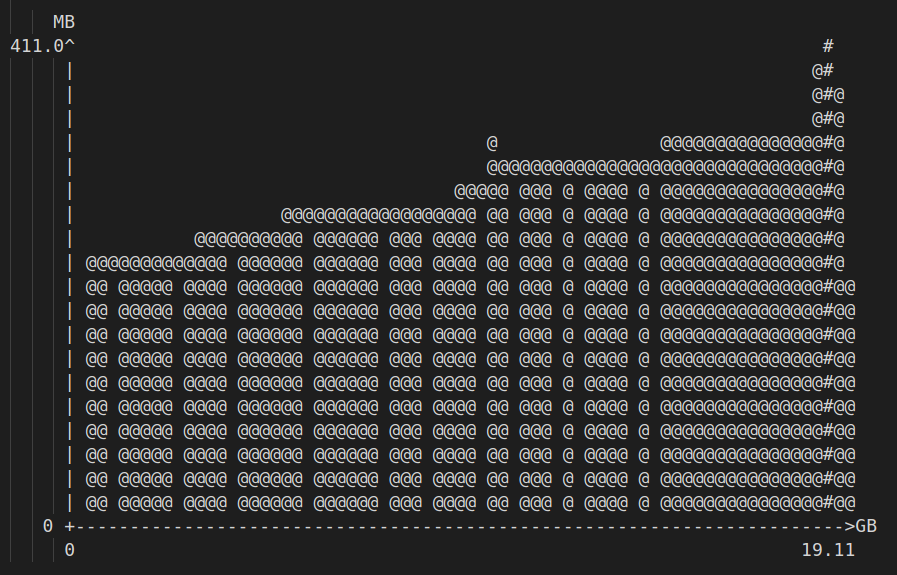
\includegraphics[scale=0.4]{mem_milan_par.png}
    \caption{Memory occupation of parallel A* with Milan grid}
    \label{mem-par-milan}
\end{figure}


\begin{figure}
    \centering
    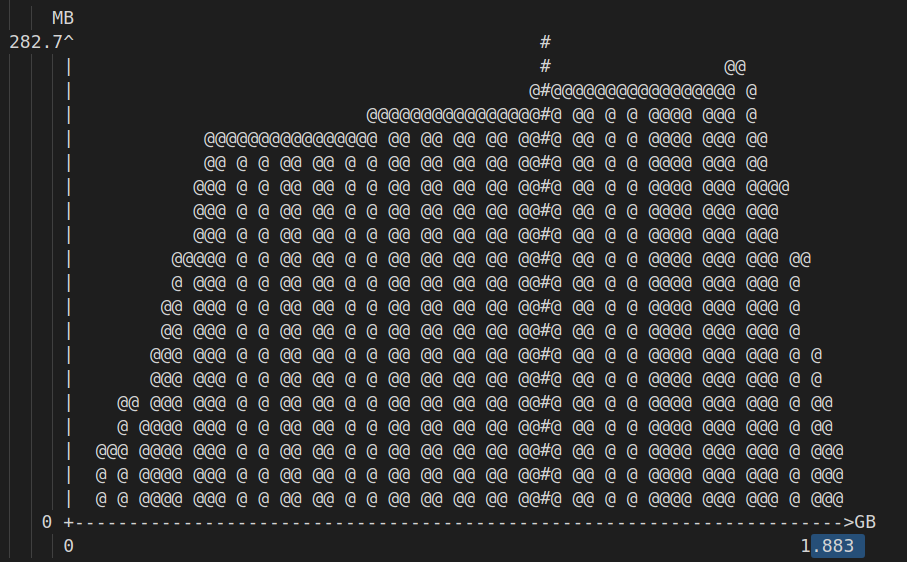
\includegraphics[scale=0.4]{mem_milan_seq.png}
    \caption{Memory occupation of sequential A* with Milan grid}
    \label{mem-seq-milan}
\end{figure}

As expected the occupation of the sequential A* is lower, since it has only one OPEN and CLOSED sets and it does not need to allocate additional structures for threads communication and synchronization.
It can be also noticed the difference between the sum of all the allocation made by the two algorithms.



\begin{figure}
    \centering
    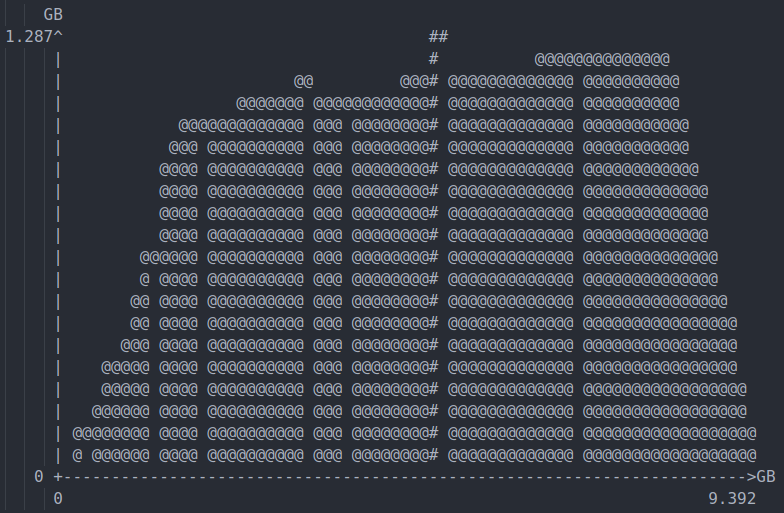
\includegraphics[scale=0.4]{mem_map_seq.png}
    \caption{Memory occupation of sequential A* with large map}
    \label{mem-seq-map}
\end{figure}

\begin{figure}
    \centering
    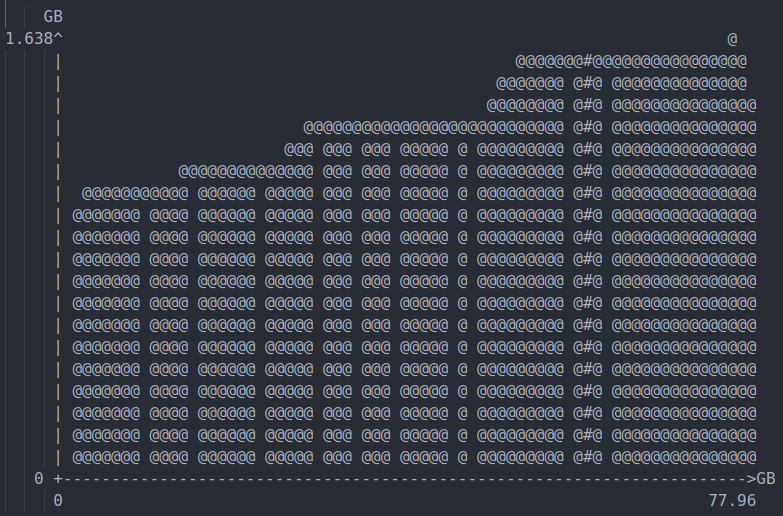
\includegraphics[scale=0.4]{mem_map_par.png}
    \caption{Memory occupation of parallel A* with large map}
    \label{mem-par-map}
\end{figure}


To ensure that are not memory leak we used an option of the Valgrind tool which keep track of all heap blocks issued in response to calls to malloc.
As shown by the the Figure \ref{mem-leak-milan} the algorithm does not have any memory leakage.

\begin{figure}
    \centering
    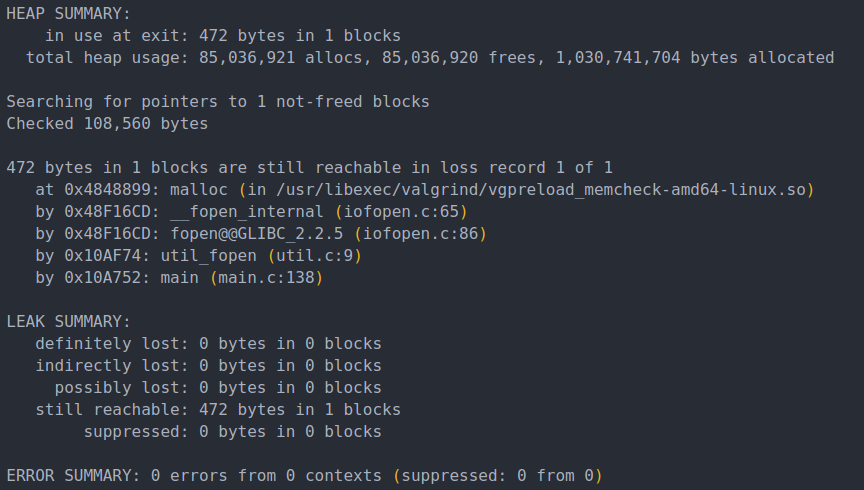
\includegraphics[scale=0.4]{mem_leak_report.png}
    \caption{Valgrind output of memory leak of parallel A* with Milan grid}
    \label{mem-leak-milan}
\end{figure}


